\documentclass[12pt,letterpaper,noanswers]{exam}
\usepackage[usenames,dvipsnames,svgnames,table]{xcolor}
\usepackage[margin=0.9in]{geometry}
\renewcommand{\familydefault}{\sfdefault}
\usepackage{multicol}
\pagestyle{head}
\header{AM 108 Class 28}{}{Maps and dimension}
\runningheadrule
\headrule
\usepackage{graphicx} % more modern
\usepackage{amsmath} 
\usepackage{amssymb} 
\usepackage{hyperref}
\usepackage{tcolorbox}

\begin{document}
 \pdfpageheight 11in 
  \pdfpagewidth 8.5in

\noindent 




\begin{itemize}
\itemsep0em
\item You have a project weekly log due Friday (and again next Friday).
\item There is a 2d system analysis due today.
\item There is a new skill check for Friday.
\item The Quiz 02 Follow Up is due Mon Nov 23rd.  The retake, if assigned to you, is due Thurs Dec 3rd.  Request a different due date via private message on Piazza, if needed.
\item There is a pre-class assignment for Monday.
\end{itemize}

\hrule
\vspace{0.2cm}



\noindent\textbf{Teams}




\noindent \textbf{Teams 5 and 6}: Post screenshots of your work to the course Google Drive today.  Include words, labels, and other short notes that might make those solutions useful to you or your classmates.  Find the link in Canvas (or here: \url{https://drive.google.com/drive/u/0/folders/1GcpwvKHD4tMecpFQ4lNxN_r5Ylj7YHbd})


\vspace{0.2cm}

\hrule
\vspace{0.2cm}


\noindent\textbf{Big picture}

Attractors in chaotic systems have a \emph{fractal} structure.  We are looking at a few examples of fractals, and also examining how people talk about the dimension of a fractal set.

\vspace{0.2cm}
\hrule
\vspace{0.2cm}

\noindent \textbf{Extra vocabulary / extra facts:}
\begin{tcolorbox}

A line segment of length $1$ can be covered by $n$ 'boxes' of length $1/n$, while a square in the plane of side length $1$ can be covered by $n^2$ boxes of side-length $1/n$.  Let $N(\epsilon)$ be the number of boxes needed to cover a set $S$ when the boxes are of side length $\epsilon$.  $N(\epsilon) = c\left(\frac{1}{\epsilon}\right)^d$.  In the limit, as $\epsilon \rightarrow 0$, $d$ is called the \textbf{box-counting dimension} of the set $S$.  $\text{boxdim}(S) = \lim_{\epsilon\rightarrow 0} \ln N(\epsilon)/\ln(1/\epsilon)$ (when the limit exists).
\end{tcolorbox}

\vspace{0.2cm}
\hrule
\vspace{0.2cm}

\vspace{0.2cm}
\hrule
\vspace{0.2cm}

\noindent\textbf{Skill Check C29 practice}
\begin{questions}
\item Retake of skill check C26.

\item The image below is an excerpt of the orbit diagram for the logistic map, given by $x_{n+1} = f(x_n)$ for $f(x) = rx(1-x).$

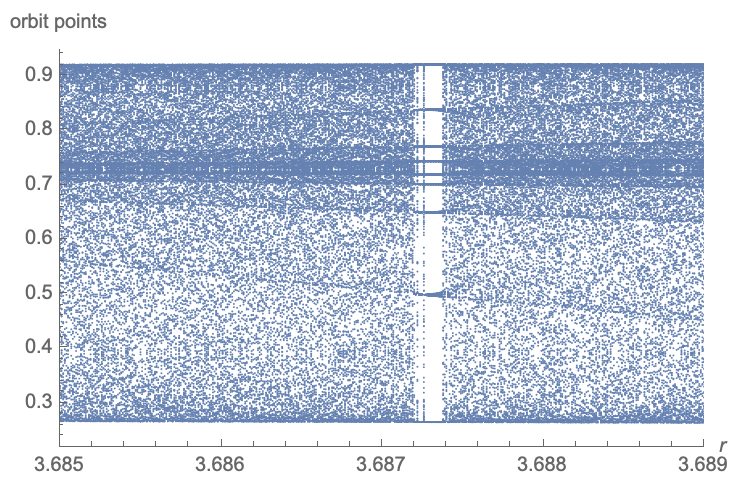
\includegraphics{img/C28-2019-11-11p2.png}

There is a very visible ``periodic window'' in the map.  Within the window, a number of different periods of periodic orbit occur.

\begin{itemize}
    \item Identify the lowest period of periodic orbit visible in the window.
    \item Provide an estimate of a parameter value where that period of orbit is occurring.
    \item The periodic orbit you identified above would manifest as $k$ (stable) fixed points in some map.  Provide an expression for that map.
\end{itemize}  

\begin{tabular}{|c|c|c|}
\hline
period & parameter value & expression for map \\
\hline
& &\\
& &\\
& &\\
\hline
\end{tabular}
\end{questions}

\vspace{0.2cm}

\hrule
\vspace{0.2cm}

\noindent\textbf{Skill Check C29 Practice Solution}


There's a clear periodic window at around $p = 3.6873$ or so.

I see nine somewhat horizontal lines in the window, so the lowest period visible in there is nine points (there are going to be period-doubling bifurcations within the window: 9 to 18 to 36 to etc, in a period-doubling cascade, but 9 is the lowest).

These nine points will be nine fixed points of $f^9(x)$ (period-1 and period-3 points will also be fixed points of that map.)

\vspace{0.2cm}

\hrule
\vspace{0.2cm}


\noindent\textbf{Questions}

\noindent \ \ 0.  Share a type of music (or a song you enjoy) with your team, and write your names on the slide.

\begin{questions}




\question (Our first 2D map) 

The Baker's map is given by
\[B(x_n,y_n)= (x_{n+1},y_{n+1}) = \left\{ \begin{array}{c c} (2x_n, ay_n) &\mbox{ for } 0\leq x_n \leq \frac{1}{2} \\ (2x_n-1, ay_n+\frac{1}{2}) &\mbox{ for } \frac{1}{2} \leq x_n \leq 1 \end{array} \right. .\]  It is illustrated by Figure 12.1.4 of the text, shown below.

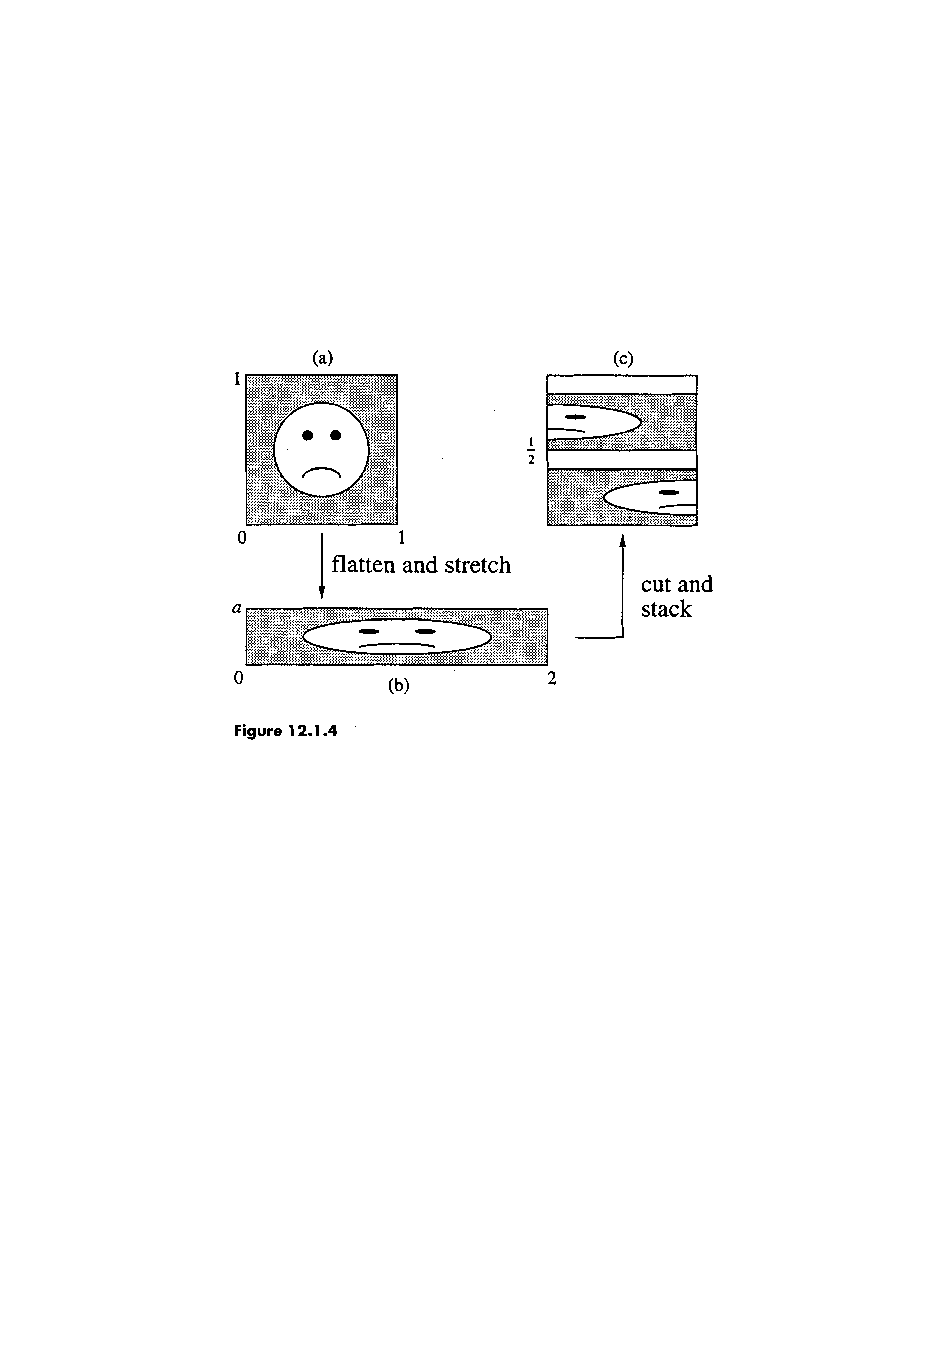
\includegraphics[scale=1]{img/C25baker.pdf}

The Baker's transformation is a simple model with chaotic dynamics.  We can reason about the long term behavior under this map by thinking geometrically, or by rewriting the map as a shift map on a sequence of numbers.

% This map can be expressed via \textbf{symbolic dynamics}, or dynamics that are represented via shifts on sequences of numbers.
\begin{parts}
\item $B(x_n, y_n)$ is equivalent to the procedure of stretching by $2$, flattening by $a$, then cutting and stacking, that is shown in the figure.  Convince yourself and your team that this is the case.  \emph{For $a<1/2$ there is are blank horizontal spaces present after stacking.  These are regions of the unit square that nothing in the original domain maps to.}
\item Sketch what will happen after one more iterate of the map shown in the figure.  \emph{Include the face and the bands of empty space (white space on this sheet)}.
\item This process might remind you of forming the Cantor set.  Sketch some representation of the limiting set.  How would you describe this set?   

\item Explain why we can't use similarity dimension to determine the dimension of the limiting set.
\item The box dimension is another way to compute fractal dimension.  Box dimension is given by
$d = \lim_{\epsilon \rightarrow 0} \frac{\ln N}{\ln \frac{1}{\epsilon}}$ where $N$ is the number of boxes needed to cover the set and $\epsilon$
is the side length of the boxes.  Compute the box dimension for the limiting set of the Baker's map.

\emph{Cover the $n^{th}$ iterate of the map with square boxes
of side length $a^n$.  Note that the first iterate has $2$ stripes and the second has $4$.  }
\item In the case $a = \frac{1}{2}$, your box dimension should be $2$ because the map is area preserving (and not leading to a fractal).  Check that this is the case.

\end{parts}

\question
\begin{parts}
\item (12.1.5) Much of the analysis people do on maps is done by understanding the map via sequences of numbers.  This process is called \emph{symbolic dynamics}, and is a common focus for pure mathematics courses in dynamical systems.  

For the area preserving Baker's map, consider a binary representation of a point in the unit square:
\[ (x,y)_2 = (0.a_1 a_2 a_3 ...,\ 0.b_1b_2b_3...)\] where $a_1=0$ indicates the point has $0\leq x < \frac{1}{2}$ and $a_1 = 1$ indicates the point
has $\frac{1}{2} \leq x < 1$.  Given the binary representation of $(x,y)$, find the binary representation of $B(x,y)$.

\textit{Multiplying a coordinate by $2$ has the effect of shifting the decimal place once to the right.}
\item Represent the point $(x,y)$ as $... b_3 b_2 b_1 . a_1 a_2 a_3 ...$.  In this notation, what is $B(x,y)$?
\item Use the binary version of the map to show that $B$ has a single period-2 orbit.  Plot the locations of the two points involved in the orbit
in the unit square.
\end{parts}

\end{questions}

\eject
\begin{enumerate}




\item
\begin{enumerate}
 \item For the unit square, consider the sets \[S_0=\{(x,y): 0\leq x < \frac{1}{2}, 0\leq y < 1\}\]
 and \[S_1=\{(x,y): \frac{1}{2} \leq x < 1, 0\leq y < 1\}.\]  These are right half ($S_1$) and the left half ($S_0$) of the unit square.
 
 Under the action of the map, points in $S_0$ are mapped to $(2x, ay)$.  This stretches $S_0$ in the $x$ direction, by a factor of two so that it takes up the whole range $0\leq x < 1$.  In addition, $y$ is squished by a factor of $a$.  This is the same thing as what happens to $S_0$
 if we stretch by $2$, flatten by $a$, and then cut halfway across, as $S_0$ is not impacted by the cut/stack step of the procedure.

$S_1$ is also stretched and flattened.  The $(\frac{1}{2},0)$ corner of $S_1$
 is placed at $(0, \frac{1}{2})$, setting the placement of the whole stretched/flattened set.  This is also equivalent to
 what happens to the set $S_1$ under the flattening/stretching and cutting/stacking procedure shown in the image.
 \item 
 
 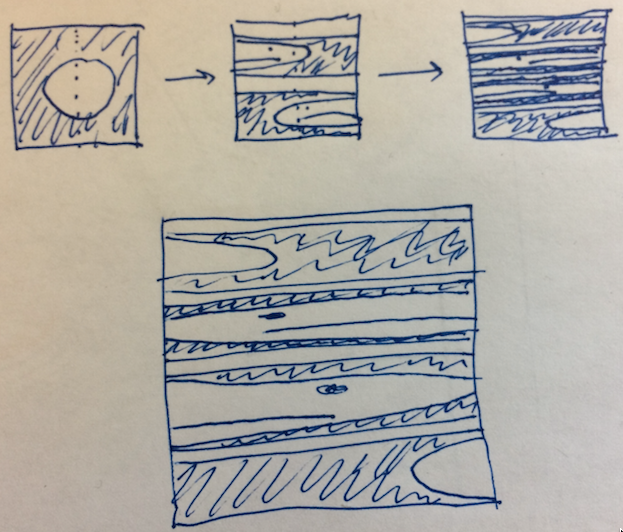
\includegraphics[width=4in]{img/C22bakers.png}
 
 \item The limiting set is like a Cantor set cross a line segment (so stripes spaced like a Cantor set).  Its dimension should be approximately $1+$ the dimension of the Cantor set, because it has an extra dimension.  \item The set isn't self similar: the length never changes, just the width shrinks. Similarity dimension doesn't make sense here.
 \item At the nth iterate, we have $2^n$ stripes and need $\frac{1}{a^n}$ boxes to cover a single stripe (stripes are of width $a^n$ and of length $1$), so there
 are $\left(\frac{2}{a}\right)^n$ boxes being used and the box size is $a^n$.  
 $d = \lim_{n\rightarrow\infty} \frac{\left(\frac{2}{a}\right)^n}{\ln \frac{1}{a^n}} = 1- \frac{\ln 2}{\ln a} = 1+ \frac{\ln 2}{\ln (1/a)}.$
 \item If we plug in $a = \frac{1}{2}$ we have $d = 1+ \frac{\ln 2}{\ln 2} = 2$.
 \end{enumerate}
 
 \item
 \begin{enumerate}
 \item The $x$ coordinate is right shifted by the stretch (the map multiplies it by $2$), so it becomes $a_1.a_2a_3a_4...$.
 Cutting and stacking turns it into $0.a_2a_3a_4...$.  For the $y$ coordinate, it depends on the $x$ coordinate.
 If $a_1 = 0$ then $y$ becomes $0.0b_1b_2...$ while if $a_1 = 1$ then $y$ becomes $0.1b_1b_2...$.  So
 $(0.a_1a_2a_3,0.b_1b_2b_3) \mapsto (0.a_2a_3...,0.a_1b_1b_2...)$.
 \item $...b_3b_2b_1.a_1a_2a_3... \mapsto ...b_2b_1a_1.a_2a_3a_4...$ so the map acts as a shift map on
 this representation.
 \item For a period-$2$ orbit, we are looking for a binary number that returns to itself after two shifts.  These are the repeating fractions
 $...101010.101010...$ and $...010101.010101...$.  Their coordinates are given by 
 $x = \frac{1}{2}+\frac{1}{8}+..., y = \frac{1}{4}+\frac{1}{16}+_...$ and vice versa.
 Thus $x - \frac{1}{4}x = \frac{1}{2} \Rightarrow x_1 = \frac{2}{3}$ and $y-\frac{1}{4}y = \frac{1}{4} \Rightarrow y = \frac{1}{3}$.  The points are
 $(\frac{2}{3},\frac{1}{3})$ and $(\frac{1}{3},\frac{2}{3})$. 
 \end{enumerate}
\end{enumerate}

\end{document}